\documentclass[12pt]{article}
\usepackage{tabularx}
\usepackage[utf8x]{inputenc}
\usepackage{indentfirst}
\usepackage{amsthm}
\usepackage{amsfonts}
\usepackage{amssymb}
\usepackage{tikz}
\usepackage{array}
\usepackage{geometry}
\usepackage{mathtools}
\usepackage{chngcntr}
\usepackage{caption}
\usepackage{subcaption}
\usepackage{setspace}
\usepackage{enumitem}
\usepackage{siunitx}
\usepackage{color, colortbl}

\geometry{
	a4paper,
	lmargin=3cm,
	rmargin=2cm,
	tmargin=3cm,
	bmargin=2cm
}
\usetikzlibrary{arrows, shapes, automata, petri, positioning}

\theoremstyle{definition}
\newtheorem{theorem}{Theorem}
\counterwithin*{theorem}{subsection}
\newtheorem{definition}{Definition}
\counterwithin*{definition}{subsection}
\newtheorem{remark}{Proposition}
\counterwithin*{remark}{subsection}
\newtheorem{lema}{Lema}
\newtheorem{algo}{Algorithm}
\counterwithin*{algo}{subsection}

\definecolor{Gray}{gray}{0.9}
\graphicspath{{./images/}}

\counterwithin*{lema}{subsection}
\linespread{1.3}

\begin{document}
	\begin{titlepage}
		\begin{center}
			\vspace{1cm}
			``ALEXANDRU IOAN CUZA" UNIVERSITY OF IAȘI
			\
			\\
			\begin{large}
				\textbf{FACULTY OF COMPUTER SCIENCE}\\
			\end{large}
			\vspace{2.5cm}
			
\includegraphics{fii.png}
			\
			\\
			\vspace{1cm}
			MASTER'S THESIS
			\begin{large}
				\
				\\
				\vspace{1.5cm}
				\textbf{Human Gait Recognition using Deep Neural Networks}
			\end{large}
			\\
			\vspace{1.5cm}
			\textbf{proposed by}
			\\
			\vspace{1.5cm}
			\textit{\textbf{Rareș-Alexandru Stan}}
			\\
			\vspace{2cm}
			\textbf{Session:} \textit{February, 2020}
			\\
			\vspace{1.5cm}
			\textbf{Scientific Coordinator}
			\
			\\
			\
			\\
			\textbf{Lect. Dr. Ignat Anca}

		\end{center}
	\end{titlepage}
	\clearpage

	\begin{titlepage}
		\begin{center}
			\textbf{``ALEXANDRU IOAN CUZA" UNIVERSITY OF IAȘI}
			\
			\\
			\textbf{FACULTY OF COMPUTER SCIENCE}\\
			\vspace{6cm}
			\
			\\
			\begin{huge}
				\textbf{Human Gait Recognition using Deep Neural Networks}
			\end{huge}
			\\
			\begin{large}
				\vspace{3cm}
				\textit{\textbf{Rareș-Alexandru Stan}}
				\\
				\vspace{3cm}
				\textbf{Session:} \textit{February, 2020}
				\\
			\end{large}
			\vspace{3cm}
			\textbf{Scientific Coordinator}
			\
			\\
			\textit{\textbf{Lect. Dr. Ignat Anca}	}
		\end{center}
	\end{titlepage}

	\clearpage
	\tableofcontents
	\clearpage

	\section{Introduction}
	\vspace{1cm}

	Gait is the movement pattern of the limbs during walking over a solid surface. It varies based on speed, terrain, maneuvering or efficiency of energy. This movement is unique for each human and can be used for recognizing persons from afar, without the need of their cooperation or physical contact, whereas fingerprint, iris or facial do need the physical access or their cooperation \cite{biometrics-comparison}. Human gait is bipedal, biphasic forward propulsion of the center of gravity of the human body. This movement is the combination of alternate sinuous movements of body segments. The uniqueness of gait is due to:
	\begin{itemize}
		\item small differences in the limb movement patterns from one person to another,
		\item velocity,
		\item changes in the contact with the surface,
		\item cycles of kinetic and potential energy \cite{gait-biomecanics}.
	\end{itemize}

	Human gait recognition is the process in which a person or an automated system looks at a sequence of frames of a person walking and identifies the unique patters of the movement and matches it, with a degree of certainty, to a person that has his/shes movements known to the one making the identification.

	An automated system can do gait recognition using one or multiple of these three classes of recording the movement: Machine Vision (MV), floor sensors and wearable sensors. MV is focused on the fine movements of a persons body while walking, whereas flor or wearable sensors focus on the kinetic and potential energy cycles. Usually MV is preferred because it is effective in continuous authentication, can identify multiple people at the same time, using just one sensor, whereas the flor or wearable sensors can identify just one person at a time, and is the most non-intrusive approach.

	One of the most popular data sets for gait recognition is the CASIA-B database \cite{casia1}\cite{casia2}\cite{casia3}. It contains both videos and sets of frames, that are split into 2 parts, each containing recordings of 62 people walking. For each person we have 3 categories of footage:
	\begin{itemize}
		\item holding a shoulder bag,
		\item waring a big coat,
		\item only normal clothes on.
	\end{itemize} We preferred to use the frame sequences, rather than the videos, because they already have the silhouettes outlined and filled. Samples from each category, of the silhouettes, are shown in Figure~\ref{figure:image-categories-sample}.

	\begin{figure}[h]
		\centering

		\begin{subfigure}{6cm}
			\centering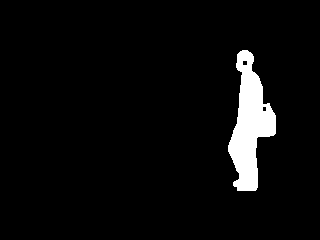
\includegraphics[width=5cm]{silhouettes/001-bg-01-090-045.png}
			\caption{Silhouette of person walking with shoulder bag}
		\end{subfigure}
		\hspace{0.5cm}
		\begin{subfigure}{6cm}
			\centering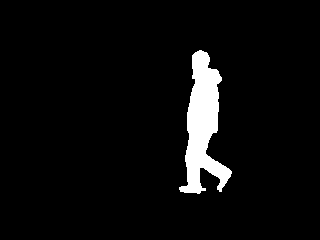
\includegraphics[width=5cm]{silhouettes/001-cl-01-090-062.png}
			\caption{Silhouette of person walking while waring big coat}
		\end{subfigure}

		\vspace{0.5cm}
		\begin{subfigure}{6cm}
			\centering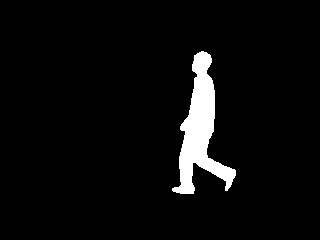
\includegraphics[width=5cm]{silhouettes/001-nm-01-090-066.png}
			\caption{Silhouette of person walking with normal clothes on}
		\end{subfigure}

		\caption{Sample images taken from all the different categories, of the CASI-B data set, filmed at 90 degrees from the subject}
		\label{figure:image-categories-sample}
	\end{figure}

	For the first tow categories we have 2 sets of sequences, called: bg-01, bg-02, cl-01 and cl-02 and for the normal clothes category we have six sets, from nm-01 to nm-06. Finally each set contains footages from 11 different angles, of only one person walking. The number of frames for each person, set and angle varies from around 40 to over 100. Each frame is a black and white image, of $300 \times 240$ pixels, where the background is black and the persons silhouette is in white. An example of a gait cycle, taken from one of the normal clothes sets is shown in Figure~\ref{figure:gait-cycle}.

	\begin{figure}[h]
		\centering

		\begin{subfigure}{6cm}
			\centering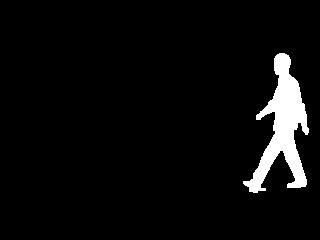
\includegraphics[width=5cm]{silhouettes/walk/001-nm-01-090-050.png}
			\caption{}
		\end{subfigure}
		\hspace{0.5cm}
		\begin{subfigure}{6cm}
			\centering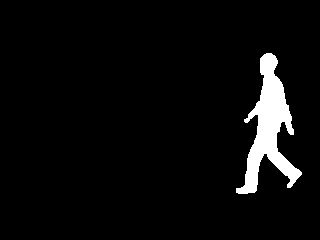
\includegraphics[width=5cm]{silhouettes/walk/001-nm-01-090-053.png}
			\caption{}
		\end{subfigure}

		\vspace{0.5cm}
		\begin{subfigure}{6cm}
			\centering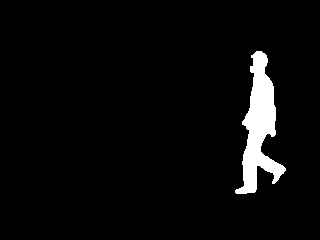
\includegraphics[width=5cm]{silhouettes/walk/001-nm-01-090-055.png}
			\caption{}
		\end{subfigure}
		\hspace{0.5cm}
		\begin{subfigure}{6cm}
			\centering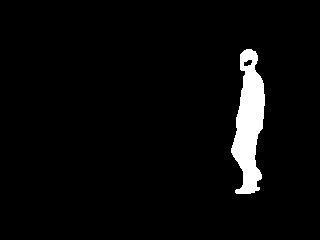
\includegraphics[width=5cm]{silhouettes/walk/001-nm-01-090-057.png}
			\caption{}
		\end{subfigure}

		\vspace{0.5cm}
		\begin{subfigure}{6cm}
			\centering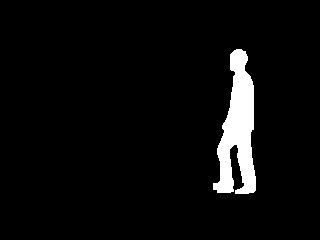
\includegraphics[width=5cm]{silhouettes/walk/001-nm-01-090-059.png}
			\caption{}
		\end{subfigure}
		\hspace{0.5cm}
		\begin{subfigure}{6cm}
			\centering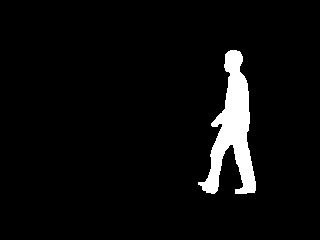
\includegraphics[width=5cm]{silhouettes/walk/001-nm-01-090-060.png}
			\caption{}
		\end{subfigure}

		\caption{Representation of gait cycle taken from CASI-B data set, filmed at 90 degrees from the subject}
		\label{figure:gait-cycle}
	\end{figure}


	We did not include in the training and evaluation of performance the bg-01, bg-02, cl-01 and cl-02 sets and focused on the nm-01 to nm-06 sets.

	In this theses we will create a system for human gait recognition using Machine Vision and Convolutional Neural Networks, that accepts a series of frames of the person walking as input and will say with a certain confidence which person was in the input. The data used for training, validating and testing our approaches is the CASIA-B database.

	\clearpage

	\section{State of the Art}
	\vspace{1cm}

	Human gait is the movement pattern of the limbs during walking. It can vary depending on the persons age, weight, how tired he is and if he is carrying extra weight. A system for recognizing persons by their walking should take all of the situations from above, to correctly identify them.

	There are three main approaches for identifying people by their gait, Machine Vision (MV), floor sensors and wearable sensors. Each of the three approaches have some disadvantages and advantages:
		\begin{itemize}
			\item MV:
				\begin{itemize}
					\item it is cheaper to implement, no need to install extra sensors, just some video cameras;
					\item can cover a wide area;
					\item it is affected if the people are wearing voluminous clothes;
				\end{itemize}
			\item Floor Sensors:
				\begin{itemize}
					\item are not affected by the clothes worn by the user;
					\item are more expensive to implement than MV;
					\item limited area for recognizing people;
				\end{itemize}
			\item Wearable Sensors:
				\begin{itemize}
					\item are not limited by a specific area;
					\item are not affected by the clothes worn by the user;
					\item you need to have physical access or to have their cooperation.
				\end{itemize}
		\end{itemize}

	In Machine Vision there are tow main approaches, model-free and model-based, where the first approach uses direct image sequences, whereas the latter needs more processing of the input sequence.

	\subsection{Model-Based Machine Vision}

	Molhema Mohualdeen and Magdi Baker \cite{gait-silhouette-nn} have proposed a model-based approach for the Gait Recognition problem using Region os Interest (ROI), Discrete Wavelet Transform (DWT), Edges, Gait Cycle and Neural Networks.
	ROI was used in the preprocessing phase to reduce data and extract the exact silhouette from each frame, by cropping. Next, in the feature extraction phase, they used DWT for multi-scale analysis, using diagonal, horizontal and vertical details of the three levels low pass and high pass filters on two dimensions DWT. Beside 3L-2D-DWT they used Edge Detection for magnitude and orientation and box technique for step and cycle length, using the with of the bounding box. Estimating the Gait Cycle was done by combining the silhouettes between the tow main phases of Gait and combining them together for each person and measuring the combination area and the width of the white shape boundary represents the step length. Classification was done using a Back Propagation Neural Network (BPNN).

	Munif Alotaibi and Ausif Mahmood \cite{gait-with-gei} propose a different type of preprocessing with a Convolutional Neural Network for classification. The processioning is done using the Gait Energy Image (GEI) \cite{gei}, defined as: $GEI(x, y)=1/s\sum_{t-1}^{s}F^t(x, y)$, where $s$ is the total number of frames representing the Gait Cycle and $F^t(x, y)$ is the silhouette of the subject at the time interval $t$. For determining the Gait Cycle it is used the bounding box changes method and the silhouettes are then resized to $140 * 140$ pixels. The Neural Network has 4 pairs of Convolution and Pooling layers, each with eight $5 * 5$ filters and eight sub-sampling maps with pooling factor $2$. For the activation function of the Convolutional layers it is used the Hyperbolic Tangent function. After the last Convolution and Pooling pair a Dense Layer with 124 nodes and SoftMax activation functions is used, to classify the data. For adding a new user to be recognized by the system, the old model is taken and froze the Convolutional and Pooling layers, so they are not changed during the new training period, and just the Dense Layer is modified, by adding a new node, and retrained.

	Hazem El-Alfy, Ikuhisa Mitsugami and Yasushi Yagi \cite{gait-with-curvature-map} build a system in which the preprocessing is done using the Gauss Map of the silhouettes and classification they use Euclidean Distance on the feature vectors between the person to be recognized and the existing database. In more details, the Gauss Maps wore done on the silhouette's surface, evaluated locally, to overcome the lack of the third dimension and made all the normal vectors point outwards the silhouette. Gauss Mapping was done on a silhouette with it's boundary extracted then smoothed using a parametric cubic spline interpolation, for it's continuity at zero, first and second order with control points being every fifth pixel of the boundary. All of the silhouettes pixels are then Distance Transformed where the distance is calculated as follows $d=max(|x_1-x_2|, |y_1-y_2|)$, where $(x_1, y_1)$ and $(x_2, y_2)$ are two distinct pixels from the image and then are computed the contour lines of the distance map. After this the image is divided in a regular grid and for each cell in computed a histogram of all the normal vectors in that contour cell. All of the cell are combined in a feature vector and it is repeated for all contours in that image. Last all the feature vectors for that image are merged into the final feature descriptor, the NDM. All of the NDMs from a full gait cycle are integrated together, using their average for the aggregate cycle descriptor. Over this aggregated feature vector the Euclidean Distance is calculated.

	\subsection{Model-Free Machine Vision}

	In Model-Free approaches, the input is mostly leaved intact, only small changes to normalize and sanitize it are done and let the Machine Vision algorithms decide what features to extract from the given data.

	One such model is proposed by Wolf et al \cite{Wolf2016MultiviewGR}, using 3D Convolution to represent the passing of time. The network is comprised of 7 convolution and pooling payers, using $3 \times 3 \times 3$ filter size and 3, 64, 128, 128, 256, 256 and 512 chanel from layer 1 to 7. The pooling layers generally have $2 \times 2 \times 2$ dimension, with layer 1 and 3 being exceptions, with size $2 \times 2 \times 1$, to avoid collapsing to early the time dimension. After the convolution phase of the network, tow dense layers of 4096 nodes are used for classification and a final layer with softmax for labeling the output. The input for the neural network is a Tensor with the following dimensions $192 \times 128 \times 16$, where the last dimension is time and first two are the sizes of each frame.

	Because the CASIA-B database has very few training instances, for a deep neural network, Wolf et al \cite{Wolf2016MultiviewGR} have extended it by slicing the video in multiple sequences of 16 frames. The split sequences are overlapping so the network does not associate a specific pose from the first frame with a person, but the walking sequence. When splitting for a 50 frames video, the following sets of images are obtained: (1-16), (2, 17), $\hdots$ , (35, 50). For each RGB image they transformed the 3 channel into a grayscale one and the next two optical flow for the $x$ and $y$ direction, so to augment the input data with additional features, and not just using the extracted feature/features for classification.

	Thapar Daksh, Aggarwal Divyansh, Agarwal Punjal and Nigam Aditya \cite{VGR-Net} propose a Hierarchically Generalized Multi-View Architecture, which takes as input a Tensor of shape $16 \times 112 \times 112$, with all the convolution layers having ReLU activation. The network is composed of tow main parts: angle prediction and classification using neural networks trained only for one specific angle. Voting is done on the outputs of all the angle specific networks. The first network uses part of the convolution layers from a pre-trained network and then passed to 2 dense layers, each of 4096 nodes and an output layer with 11 nodes, one for each angle in the data set. For the angle specific classification the same convolution layers are used, but followed by 7 dense layers, of 4096 nodes and an output layer for labeling the output. The dense layers use the ReLU activation and the output ones use softmax.

	After the model is trained Thapar Daksh, Aggarwal Divyansh, Agarwal Punjal and Nigam Aditya \cite{VGR-Net} fine-tuned it by using stereoscopic images. The images are obtained by combining tow consecutive silhouette frames and highlighting the differences in red or green, while keeping the common parts of the silhouette white. The difference from the first frame is colored green, while the difference for the second frame is colored red, to obtain something similar to stereoscopic images. Fine-tuning the two stage model using these augmented images further improved the performance of the model, beating the existing state of the art, from Wolf et al \cite{Wolf2016MultiviewGR}, on almost all view angles ($0^\circ$, $18^\circ$, $36^\circ$, $54^\circ$, $108^\circ$ and $180^\circ$).

	\subsection{Wearable Sensors}

	Qin Zou, Yanling Wang, Qian Wang, Yi Zhao and Qingquan Li \cite{smartphone-gait} have used the data provided by the accelerometer and gyroscope from smartphones, that people wear un themselves, for identification. After the data is collected, it is partitioned in steps, for better classification, and further processed to remove the influence of the phones position while it is worn. The network used has both Convolution and Recurrent networks and the output of both is concatenated and fed to a dense network. The CNN takes as input the data from the three axis accelerometer and three axis gyroscope as one input set. The network is structured as followed:
	\begin{itemize}
		\item convolution with 32 filters of $1 \times 9$, obtaining a feature map of size $6 \times 64 \times 32$,
		\item pooling with filter size $1 \times 2$,
		\item convolution with 64 filters of $1 \times 3$, obtaining a feature map of $6 \times 32 \times 64$,
		\item convolution with 128 filters of $1 \times 3$, obtaining a feature map of $6 \times 32 \times 128$,
		\item pooling with filter size $1 \times 2$,
		\item convolution with 128 filters of $6 \times 1$, obtaining a feature map of $1 \times 16 \times 128$.
	\end{itemize}

	The first convolution later and all the pooling layers used a stride of 2.

	\clearpage

	\section{Contributions}
	\vspace{1cm}

	The two classes of methods used for Gait Recognition using Machine Vision are: Model-Base and Model-Free. In the former class there are methods that heavily preprocess the input data or extract features that are meant to be used for classification, done by a machine learning algorithm, whereas the latter uses the base data, only with little preprocessing meant to clean and sanitize the input and the machine learning algorithm will extract what features that it sees fit for classifying the data. In this theses we have tried both Model-Based and Model-Free approaches for Human Gait Recognition and obtained the best results with one of the Model-Free approaches.

	For training and testing the CASIA-B database \cite{casia1}\cite{casia2}\cite{casia3} was used, as it already has the silhouettes extracted from the videos, which gave us the possibility to focus on the recognition methods. We have used the first part of the database, which included silhouettes for 62 people, of the 124 total. The data sets has been split in three categories: training, nm01-nm04, validation nm-05 and testing nm-06. Each set has a specific purpose, described bellow:
	\begin{itemize}
		\item the training set is the one with which the Neural Networks will learn to extract the needed features for proper classification, it being fed to the network and if the output is wrong, the algorithm will self adjust in a way to correct the misclassified inputs;
		\item the validation data set is used to make sure that the Neural Network does not overfit for the specific training input, but instead generalizes for unseen data, as seen in Figure~\ref{figure:overfitting-example};
		\item the final set of data, the testing set, is used for evaluating the models, after the training is finished, for this one the algorithm output is just compared with the expected output and the final accuracy is obtained.
	\end{itemize}

	\begin{figure}
		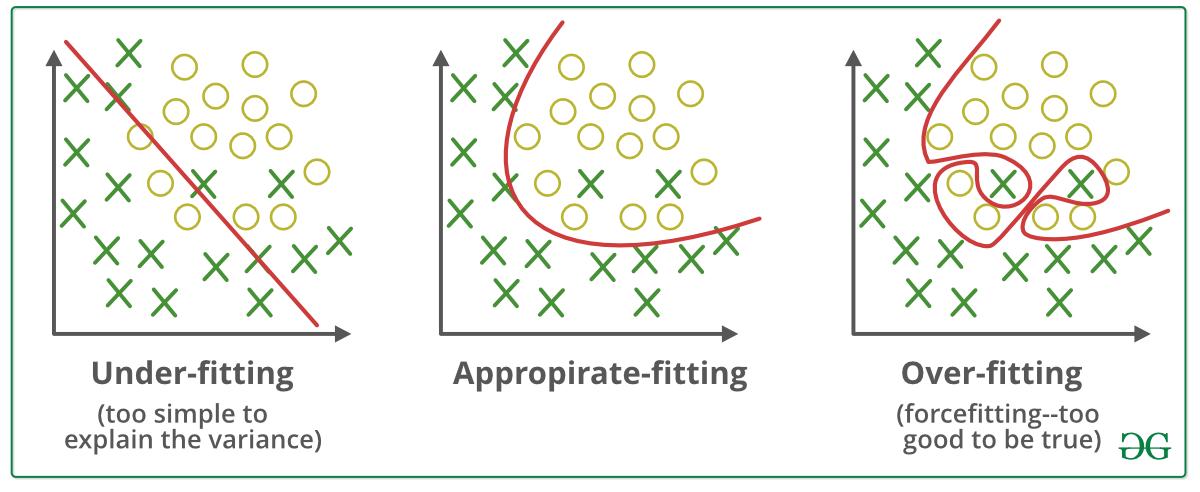
\includegraphics[width=\textwidth]{overfitting-example.png}
		\caption{Comparison of underfitting, overfitting and optimum models \cite{overfitting-example-image}}
		\label{figure:overfitting-example}
	\end{figure}

	The first model we tried, classified as a Model-Based approach, had the input images cropped, smoothed and then a surface curvature metric extracted from the silhouette and then classified using a Convolutional Neural Network In this model the CNN was not only used to extract features from images, but also extract features from the movement between frames. To express movement or temporality using CNNs, there needs to be added an additional dimension to the input, representing a sequence of frames. Through surface curvature metric we refer to a function that can map the shape, position and altitude, from an image with three dimensional objects, to a numerical value, for each pixel in the original image. Smoothing refers to the process of removing noise or fine-scale structures from images, resulting in a less jagged edges and smooth curves/transitions.

	The next models, that are classified as Model-Free approaches, have the input images centered around the silhouette and cropped, then fed to either classic Convolutional Neural Networks (CNN) or combinations of CNN and Recurrent Neural Network (RNN) \cite{rnn} for classification. With these models we explore the classification and feature extraction from movement through time is done by different passage of time representations. One such representation is achieved using a third dimension for Convolution, described in the Model-Based approach. A second method of representation is with using memory, like in Recurrent Networks, so each node can chose when to recall certain features from the past inputs of the series. This approach has very good results in language processing and generation, being able to recall themes, subjects or events, described in past inputs.

	Finally a comparison between all the trained models, based on the percentage of correctly classified frame sequences from the testing data set, which has not been used in training, database augmentation or overfitting prevention.

	When evaluating the performance of our models, the testing data set is used, by feeding each frame set one at a time and comparing the correct label with the label with the highest confidence of the network output, this method is also known as Rank-1 Identification Rate. All the correct and incorrect classifications are counted and the accuracy is calculated in percentages as follows: $\frac{C_T}{C_T + W_T}$, where $C_T$ is the total number of input sequences correctly labeled, by the model, and $W_T$ is the total number of the inputs classified incorrectly. $C_T + W_T$ give the total number of the input sequences from the testing set of data.

	\clearpage

	\section{Approach}
	\vspace{1cm}

	In the first part of this chapter we will explain what the shape index represents and how Convolutional Neural Networks and Recurrent Neural Network classify data. In the second part of the chapter the architectures and preprocessing used for the Model-Based and Model-Free approaches will be presented.

	\subsection{Shape Index}
	The shape index measures the local curvature, derived from the eigen values of the Hessian, defined by Koenderink and van Doorn \cite{shape-index}. It can be used to find structures based on their apparent local shape. It maps to values in the range $[-1, 1]$, representing different shape types. It is defined as follows:

	\begin{equation*}
	s=\frac{2}{\pi}*\arctan{\frac{k_2+k_1}{k_2-k_1}} \;\;\;\;  (k_1 \geq k_2)
	\end{equation*}

	Here $(k_1, k_2)$ are polar coordinates described by $k_{1,2}^2-2H_{k_{1,2}}+K=0$, where $H$ is the mean curvature, measuring the spread of normals for the points of infinitesimal arcs, divided by the arch length and averaged over all surfaces, and $K$ is the Gaussian curvature, specifying the spread of normals.

	\subsection{Neural Networks}

	Neural Networks (NN) are a collection of connected nodes, name neurons, that for a node $j$, at the time interval $t$, with input  $p_j(t)$, consist of:
	\begin{itemize}
		\item an activation $a_j(t)$,
		\item a threshold $\theta_j$,
		\item an activation function $f$ that computes the new activation at time $t+1$ from $a_j(t), \theta_j$ and the input $p_j(t)$, resulting $a_j(t+1)=f(a_j(t), p_j(t), \theta_j)$,
		\item and an output $o_j(t)=f_{out}(a_j(t))$
	\end{itemize}
	and with a propagation function, that computes the input $p_j(t)$, for node $j$, from $o_i(t)$ of predecessor neurons and has the form $p_j(t)=\sum_io_i(t)*w_{ij} + w_{0j}$, where $w_{0j}$ is a bias.

	Learning in Neural Networks is done by firstly feed forward the input, to compute the output of the network, for the input $x, x \in \mathbb{R}^n$, where $n$ is the size of the input vector. Secondly calculate the error of the entire network for the known input and lastly propagate the error and update the weights of each layer. The weight updating is described throw the following:
	\begin{equation*}
		w_{ij}(t+1)=w_{ij}(t)-\eta\frac{\partial C}{\partial w_{ij}}+ \xi(t)
	\end{equation*}

	where $\eta$ is the learning rate, $C$ is the cost function, and $\xi(t)$ a stochastic term. The cost function depends on the learning type and the activation function, usually in supervised learning the cost function is Cross Entropy. Back-Propagation is done for each training sample for the desired number of epochs.


	\subsubsection{Convolutional Neural Networks}

	Convolutional Neural Networks (CNN) beside the classic dense layers they have convolution and pooling layers and are primarily used for image and video related learning.
	Convolutional layers have multiple filters of fixed dimensions, randomly initialized with a uniform distribution. The $a*b$ filter is applied over the input $x$, using the dot product between the filter and sub-matrix of $x$,  with a stride $s$, and the output is added with the bias term and then the activation function is applied, this happens for all the defined filters of a convolution layer independently. Pooling layers reduce the size of the input by a specified factor, using functions like: max, average, min, etc. Pooling layers are used for enabling the following filters to look at bigger feature of the input.


	\subsubsection{Recurrent Neural Networks}

	Recurrent Neural Networks (RNN) are mostly the same as standard Neural Networks, with the added bonus of each neuron having its owen memory. The activation function is time-varied. Thanks to having internal memory for each node, RNNs can process time sequences of inputs, which makes them great for video processing, speech recognition, and generating sequences.

	One such king of RNN is Long Short-Term Memory (LSTM) \cite{lstm} which avoids the vanishing and exploding gradient. Besides the standard RNN model, they have recurrent gates, called forget gates.


	\subsection{Model-Based Approach}

	For the Mode-Based approach we used a Convolutional Neural Network which has as input a set of frames that have applied the shape index on each of them.

	Model-Based Machine Vision approaches have a preprocessing phase, in which features are extracted from the input and passed to a Machine Learning algorithm for classification.

	Because gait happens over time, we needed a way to capture the passing of time. In order to do that we used 3D Convolution, with the third dimension being time, using multiple consecutive frames.

	Before any preprocessing we sanitized the input images af follows:
	\begin{enumerate}
		\item select the first 80 frames from the database, for each angle of all the 62 people, if there are ath least that many frames in that set, otherwise take all the frames and add empty frames to the end of the series, until 80 images are reached,
		\item center the silhouette in each frame,
		\item crop all images so that only the silhouette is in the frame, with a small padding,
		\item resize the each input to $120 \times 60$ pixels.
	\end{enumerate}

	After the input is sanitized we applied the shape index algorithm for each frame, transforming it from a matrix with values $\{0, 1\}$ into a matrix with values in the range $[-1, 1]$. Then all the resulting matrixes for a persons angle are put together, in chronological order, to obtain a tensor (3D matrix), with shape $(80, 120, 60)$, 80 frames, 120 pixels heigh and 60 pixels wide frames. Each tensor is a training sample for the CNN.

	Last step is the Convolutional Neural Network, which takes as input a tensor of shape $(80, 120, 60)$ and outputs a list with confidences, for each of the 62 subjects and we will say that the CNN thinks that the input is a recording of the person with the highest confidences.
	The Model used here has four 3D convolutional layers, each followed by a 3D max pooling layer and finally a densely connected layer, of size 62, for output labeling.

	When doing convolution, values nearby are combined and evolved to express new features. When moving from a convolution layer to another, the features from the previous layer are used as input for the next one and previous features are combined to express more complex features in the current layer. The pooling layers are used to select between the features from the previous layer so after it only the important features are passed down.

	For each convolution layer, there is specified a number of filters, which will convert the input in an output with that many channels, each one having the same size as the input. Pooling happens for each chanel independently.

	In Table~\ref{table:preprocessing-CNN} all the layers are described with each ones size, number of channels and activation functions and in Figure~\ref{figure:3D-CNN} it is visually defined, with the chanel numbers omitted.

	\begin{table}[h]
		\centering
		\renewcommand{\arraystretch}{1.5}

		\caption{Description of the CNN Model used with the shape index preprocessing}
		\label{table:preprocessing-CNN}

		\begin{tabularx}{\textwidth}{XXXX}
			\textbf{Layer name} & \textbf{Size} & \textbf{No. Filters} & \textbf{Activation} \\ \hline
			3D Convolution & 10, 10, 10 & 32                   & elu                  \\ \hline
			3D Max Pooling & 2, 2, 2    & \textbf{\textendash} & \textbf{\textendash} \\ \hline
			3D Convolution & 10, 10, 10 & 16                   & elu                  \\ \hline
			3D Max Pooling & 2, 2, 2    & \textbf{\textendash} & \textbf{\textendash} \\ \hline
			3D Convolution & 5, 10, 10  & 8                    & elu                  \\ \hline
			3D Max Pooling & 2, 2, 2    & \textbf{\textendash} & \textbf{\textendash} \\ \hline
			3D Convolution & 3, 10, 5   & 4                    & elu                  \\ \hline
			3D Max Pooling & 2, 2, 2    & \textbf{\textendash} & \textbf{\textendash} \\ \hline
			Dense       & 62         & \textbf{\textendash} & softmax              \\
		\end{tabularx}
	\end{table}

	\begin{figure}
		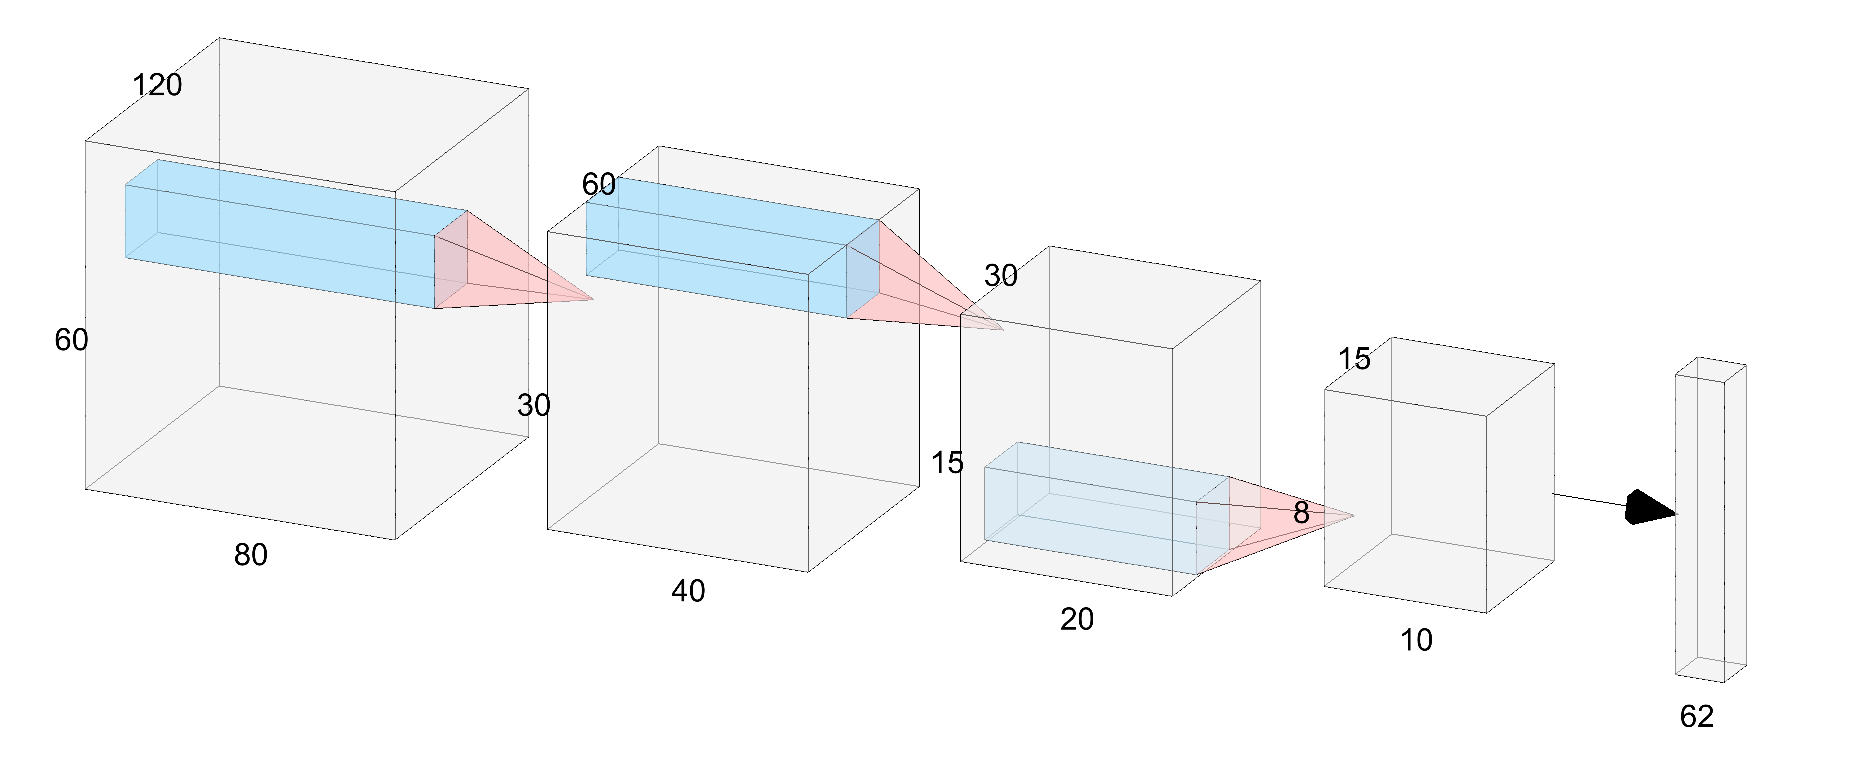
\includegraphics[width=\textwidth]{networks/3D-CNN.png}
		\caption{3D CNN visualized with the chanel numbers omitted, to better visualize the volumetric layers, generated using \cite{nn-svg}}
		\label{figure:3D-CNN}
	\end{figure}

	After training, this model proved unsuccessful, having the accuracy on both the validation and text set of inputs $\approx 1.62\%$, which is equivalent to assigning a random person to each input.

	\subsection{Model-Free Approach}

	As stated before, Model-Free approaches have little to no preprocessing, mostly to sanitize the input or reduce its size, without losing many details of features. For all the models created in this approach have little preprocessing, to normalize the size of the input and get rid of the huge empty spaces in the images as follows:
	\begin{enumerate}
		\item select the first 80 frames from the database, for each angle of all the 62 people, if there are ath least that many frames in that set, otherwise take all the frames and add empty frames to the end of the series, until 80 images are reached,
		\item center the silhouette in each frame,
		\item crop all images so that only the silhouette is in the frame, with a small padding,
		\item resize the each input to $120 \times 60$ pixels.
	\end{enumerate}

	After the cleaning and normalizing of the input data, it is feed to the Neural Network (NN). We created multiple models for the NN, to test how the size and type of layers affect the performance of the classification.

	Firstly we can se two main path in the model definition, based on how time is defined, using:
	\begin{itemize}
		\item 3D Convolution,
		\item Recurrent Neural Networks, more exactly Long Short-Term Memory (LSTM).
	\end{itemize}

	When using 3D Convolution the third dimension represents time and so when applying filters and pooling, features from different frames, different time intervals, are combined in a unique way for each person, and the dense layers, that come after the convolution, will classify each person, based on those features.

	Recurrent Neural Networks have memory, which remembers features from the past and are taken into consideration alongside with the input at the current time step.

	\subsubsection{3D Convolution}

	Seeing that the Model-Based approach gave so poor results, we tried to identify the problem and reached to the conclusion that the preprocessing with shape index somewhat transformed the input in something that the network did not find features with which to uniquely identified the people. So we dropped the shape index and used only the input normalization and the neural network, which game promising results on the validation and testing input sets of $\approx 59\%$. We iterated through a couple more models and reach a satisfactory result of 91.7\%, on the validation and testing sets, after adding an additional dense layer of 200 nodes, right after the last max pooling layer, to the original network.

	This improvement of $\approx 32.7\%$ is based on the power to extract more complex features and accentuate or remove features from the input received from the convolutional and pooling layers, of the new dense layer.

	In Table~\ref{table:dense-CNN} all the layers are described with each ones size, number of channels and activation functions and it is visually represented in Figure~\ref{figure:3D-CNN-200-Dense}, with the chanel numbers omitted.

	Preventing overfitting is a very real problem when using the CASIA-B data set \cite{casia1}\cite{casia2}\cite{casia3} due to the very few training data available, only four examples for each filming angle for all the people. A couple of examples of measures to reduce or prevent overfitting are:
	\begin{itemize}
		\item add more training data,
		\item use dropout, so that all the nodes in the network are activated,
		\item early stopping,
		\item use regularization, to control how much the weights update.
	\end{itemize}

	Out of the ones listed above we have used early stopping and adding dropout to all the layers, except the input layer. If the network did not obtain a better accuracy on the validation set than the best recorded yet, in 20 epochs, we stopped the training and run the best model on the testing set. Dropout picks at random a number of nodes, in the current layer, which will be used, so that all the nodes have equal chances to have their output evaluated and not overridden by other nodes on the same layer. In our models we chose to use a dropout on half of our nodes on each layer.

	When learning, neural networks need a function that calculates the value with which the weights of the nodes are updated, the most popular function is stochastic gradient descent, that has a fixed learning rate, used during the entire training. In later years other functions appeared that improved the stochastic gradient descent, to reduce the learning time, called AdaGrad \cite{adagrad-optimizer}, RMSProp \cite{rmsprop-optimizer} and Adam \cite{adam-optimizer}, that combines the advantages of both AdaGrad and RMSProp.
	We chose to also add the Adam optimization for the learning process.

	\begin{table}[h]
		\centering
		\renewcommand{\arraystretch}{1.5}

		\caption{Description of the CNN Model with additional dense layer highlighted}
		\label{table:dense-CNN}

		\begin{tabularx}{\textwidth}{XXXX}
			\textbf{Layer name} & \textbf{Size} & \textbf{No. Filters} & \textbf{Activation} \\ \hline
			3D Convolution    & 10, 10, 10   & 32                   & elu                  \\ \hline
			3D Max Pooling    & 2, 2, 2      & \textbf{\textendash} & \textbf{\textendash} \\ \hline
			3D Convolution    & 10, 10, 10   & 16                   & elu                  \\ \hline
			3D Max Pooling    & 2, 2, 2      & \textbf{\textendash} & \textbf{\textendash} \\ \hline
			3D Convolution    & 5, 10, 10    & 8                    & elu                  \\ \hline
			3D Max Pooling    & 2, 2, 2      & \textbf{\textendash} & \textbf{\textendash} \\ \hline
			3D Convolution    & 3, 10, 5     & 4                    & elu                  \\ \hline
			3D Max Pooling    & 2, 2, 2      & \textbf{\textendash} & \textbf{\textendash} \\ \hline
			\rowcolor{Gray}
			\textbf{Dense} & \textbf{200} & \textbf{\textendash} & \textbf{elu}         \\ \hline
			Dense          & 62           & \textbf{\textendash} & softmax              \\
		\end{tabularx}
	\end{table}

	\begin{figure}
		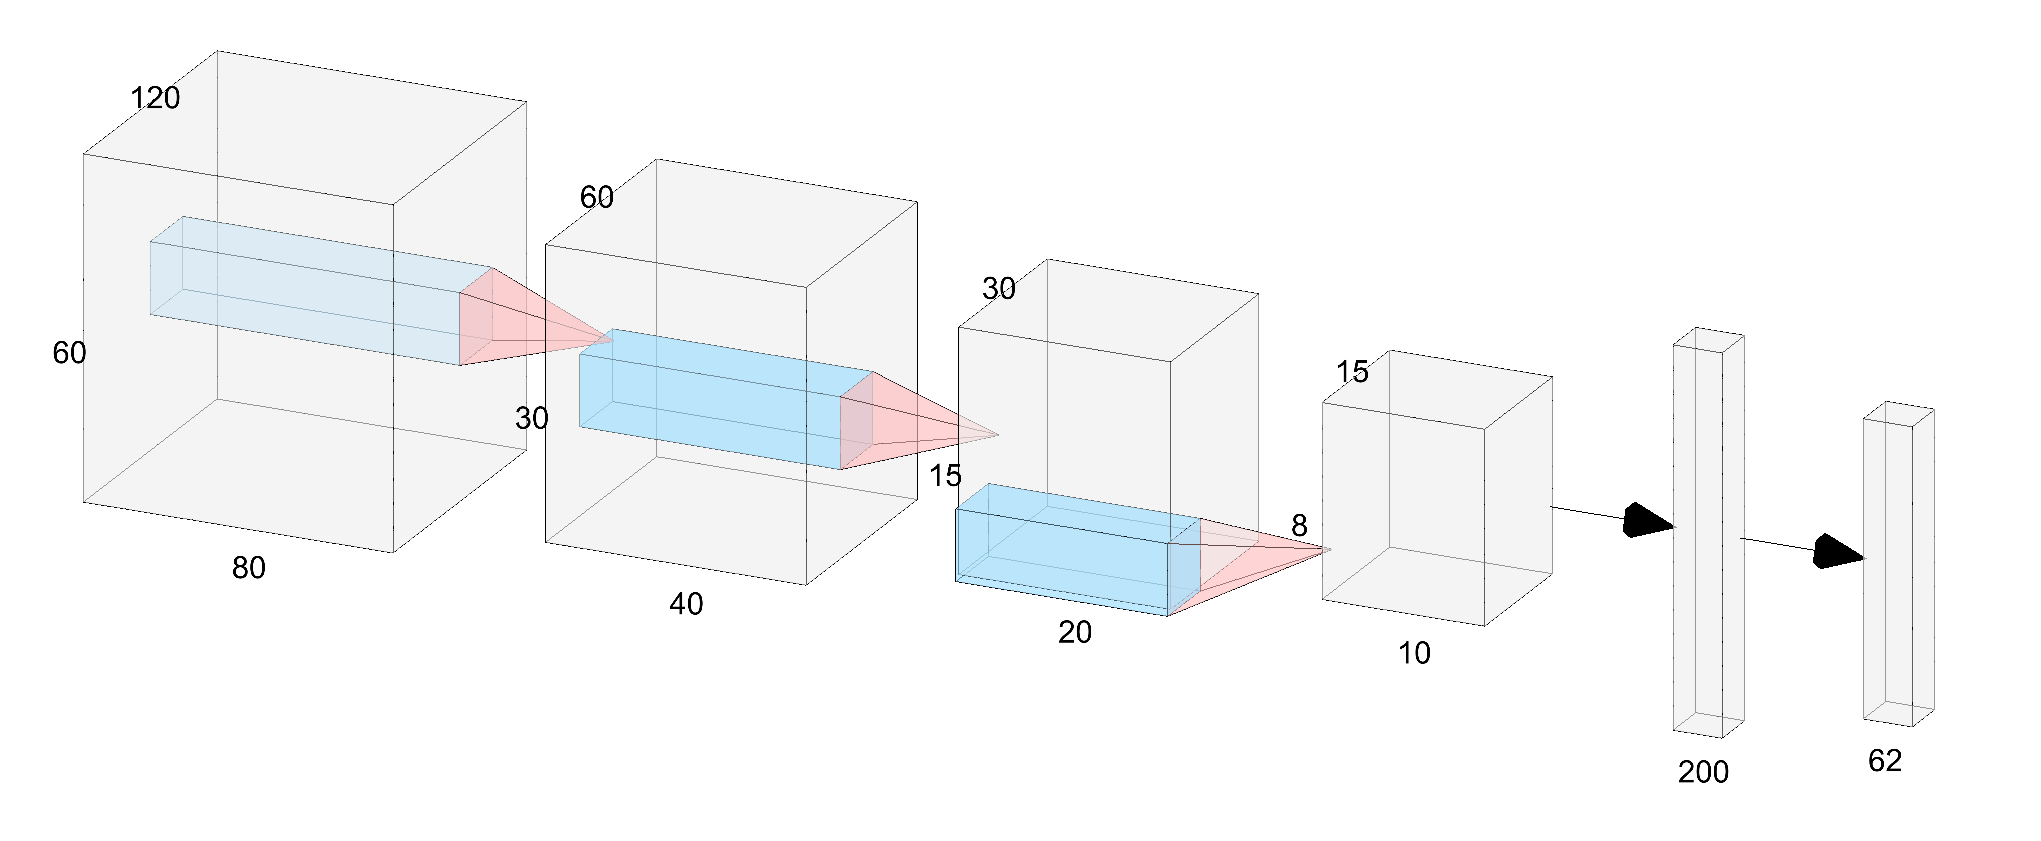
\includegraphics[width=\textwidth]{networks/3D-CNN-200-Dense.png}
		\caption{3D CNN with additional Dense layer of 200 neurons visualized with the chanel numbers omitted, to better visualize the volumetric layers, generated using \cite{nn-svg}}
		\label{figure:3D-CNN-200-Dense}
	\end{figure}

	We can see what each of the convolution layer sees for an input series of frames, by extracting the value of the activation and plotting them. By doing this with out model we obtain the following image series, shown in Figures \ref{figure:visualize-conv-1}, \ref{figure:visualize-conv-2}, \ref{figure:visualize-conv-3} and \ref{figure:visualize-conv-4}, in which we have a time sequence for each convolution chanel displayed on a row, with ten images from the time dimension, taken uniformly, for the first layer each image is taken from a multiple of eight frames, for the second layer from multiple of four, for the third layer from multiple of two and for the last one we took all the images from the time dimension. Also for the chanel we only selected four to display, selected uniformly for each layer, first chanel for each quarter set of the channels.

	\begin{figure}
		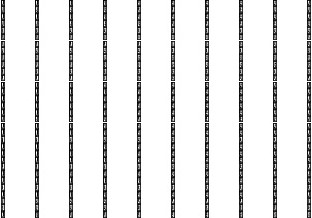
\includegraphics[width=\textwidth]{conv-see/visualization-2.jpg}
		\caption{Visualization of the first layer of convolution}
		\label{figure:visualize-conv-1}
	\end{figure}

	In the first layer, represented in Figure~\ref{figure:visualize-conv-1}, we can se that each image has a clear outline of a person walking and we can se the different phases of gait very clearly, over the time dimension. Also Each chanel emphasizes different features of the silhouette, in some of them the shape is very flat in other it gives it depth so that the network can differentiate between all the subjects.

	\begin{figure}
		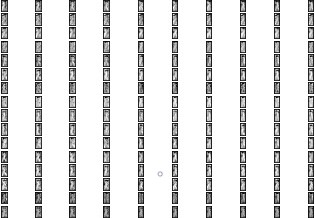
\includegraphics[width=\textwidth]{conv-see/visualization-4.jpg}
		\caption{Visualization of the second layer of convolution}
		\label{figure:visualize-conv-2}
	\end{figure}

	Moving deeper in the Convolution Layers we can see that the second layer, represented in Figure~\ref{figure:visualize-conv-2}, combines features from all the dimensions, in some of the images we see shadows of how the person moves his body while walking and also combining different parts of the body, to follow their movement together.

	\begin{figure}
		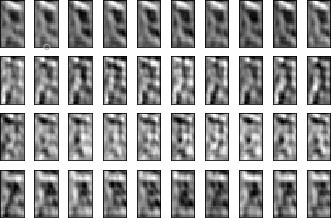
\includegraphics[width=\textwidth]{conv-see/visualization-8.jpg}
		\caption{Visualization of the third layer of convolution}
		\label{figure:visualize-conv-3}
	\end{figure}

	On the third Convolution layer, represented in Figure~\ref{figure:visualize-conv-3}, a big portion of the images do not resemble silhouettes walking, but we can distinguish the movements some patterns in the time dimension, forming clear cycles in their movement. We think that here it tries to determine the length and speed of the gait cycle.

	\begin{figure}
		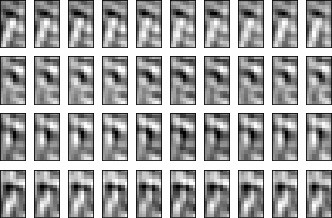
\includegraphics[width=\textwidth]{conv-see/visualization-16.jpg}
		\caption{Visualization of the fourth and last layer of convolution}
		\label{figure:visualize-conv-4}
	\end{figure}

	Lastly, on the fourth layer, represented in Figure~\ref{figure:visualize-conv-4}, no human form can be distinguished, but following the time dimension some movement patters appear, following the whole body of the subject. From this layer all the values for an array of only one dimension and given to the dense layer for classification. The power of this classification layer is very good, it being able to correctly identify $\approx 91\%$ of the subjects, only from these four movement patterns, over ten frames each.

	After training the 3D Convolutional model on all the view angles and obtained an accuracy of 91.9\% on the $90^\circ$ view angle, we have tried to specialize it on this view, by training it further on only the training samples which are taken from the $90^\circ$ angle. It needed multiple restarts until it got a better result, with 93.5\% accuracy, most of the times it overfitted the model and the performance did not improve. After this we used the same architecture and started training it from scratch only on the $90^\circ$ viewing angle. This approach also lead to overfitting, obtaining a testing accuracy of only 87\%. To increase the precision we increased the dropout rate to 0.7, but the testing concluded with a decrease in accuracy to 77.4\%. Because of the small dataset for the $90^\circ$ viewing angle and the size of the network overfitting is unavoidable, making this model unfit for specialization on only one viewing angle.

	Future work on this model could include a smarter way to select the needed frames to express the passing of time and gait movements, to help in reducing the networks size drastically.

	\subsubsection{LSTM}

	After seeing the success of the model using 3D Convolution we tried using RNN, with LSTM nodes to treat the temporality of gait. RNNs wore chosen because their success in natural language processing and generation, being able to recall events happened in the text quite early one, hoping to recall specific features that appeared in previous frames of the input.

	For doing so initially a Convolution Neural Network was created, to process and extract features for one frame, using 2D Convolution and 2D Max Pooling layers. The CNN was then used as time distributed input for a LSTM layer of 128 nodes, followed by a dense layer of 256 nodes and a dense output layer of 62 nodes.
	The LSTM layer was used for combining and selecting features across time and the first dense layer for extracting more complex features and accentuate or remove features from the input. Lastly the output dense layer labels the output, based on the features received as input.

	One of the CNN models created for the RNN consists of 4 sets of 2 2D Convolution layers followed by a 2D Max Pooling layer. The whole RNN network, with layer sizes, is described in Table~\ref{table:big-CNN-LSTM} and visually represented in Figure~\ref{figure:big-2D-CNN-LSTM-Dense}, with the chanel numbers included, because the convolutional layers are 2D, which are the most widespread and easy to represent visually.

	\begin{table}[h]
		\centering
		\renewcommand{\arraystretch}{1.5}

		\caption{Description of the CNN+RNN Model with many Convolution layers}
		\label{table:big-CNN-LSTM}

		\begin{tabularx}{\textwidth}{XXXX}
			\textbf{Layer name} & \textbf{Size} & \textbf{No. Filters} & \textbf{Activation} \\ \hline
			2D Convolution & 3, 3 & 64                   & elu                  \\ \hline
			2D Convolution & 3, 3 & 64                   & elu                  \\ \hline
			2D Max Pooling & 2, 2 & \textbf{\textendash} & \textbf{\textendash} \\ \hline
			2D Convolution & 3, 3 & 128                  & elu                  \\ \hline
			2D Convolution & 3, 3 & 128                  & elu                  \\ \hline
			2D Max Pooling & 2, 2 & \textbf{\textendash} & \textbf{\textendash} \\ \hline
			2D Convolution & 3, 3 & 256                  & elu                  \\ \hline
			2D Convolution & 3, 3 & 256                  & elu                  \\ \hline
			2D Max Pooling & 2, 2 & \textbf{\textendash} & \textbf{\textendash} \\ \hline
			2D Convolution & 3, 3 & 512                  & elu                  \\ \hline
			2D Convolution & 3, 3 & 512                  & elu                  \\ \hline
			2D Max Pooling & 2, 2 & \textbf{\textendash} & \textbf{\textendash} \\ \hline
			LSTM           & 128  & \textbf{\textendash} & tanh, sigmoid        \\ \hline
			Dense          & 256  & \textbf{\textendash} & elu                  \\ \hline
			Dense          & 62   & \textbf{\textendash} & softmax              \\
		\end{tabularx}
	\end{table}

	\begin{figure}
		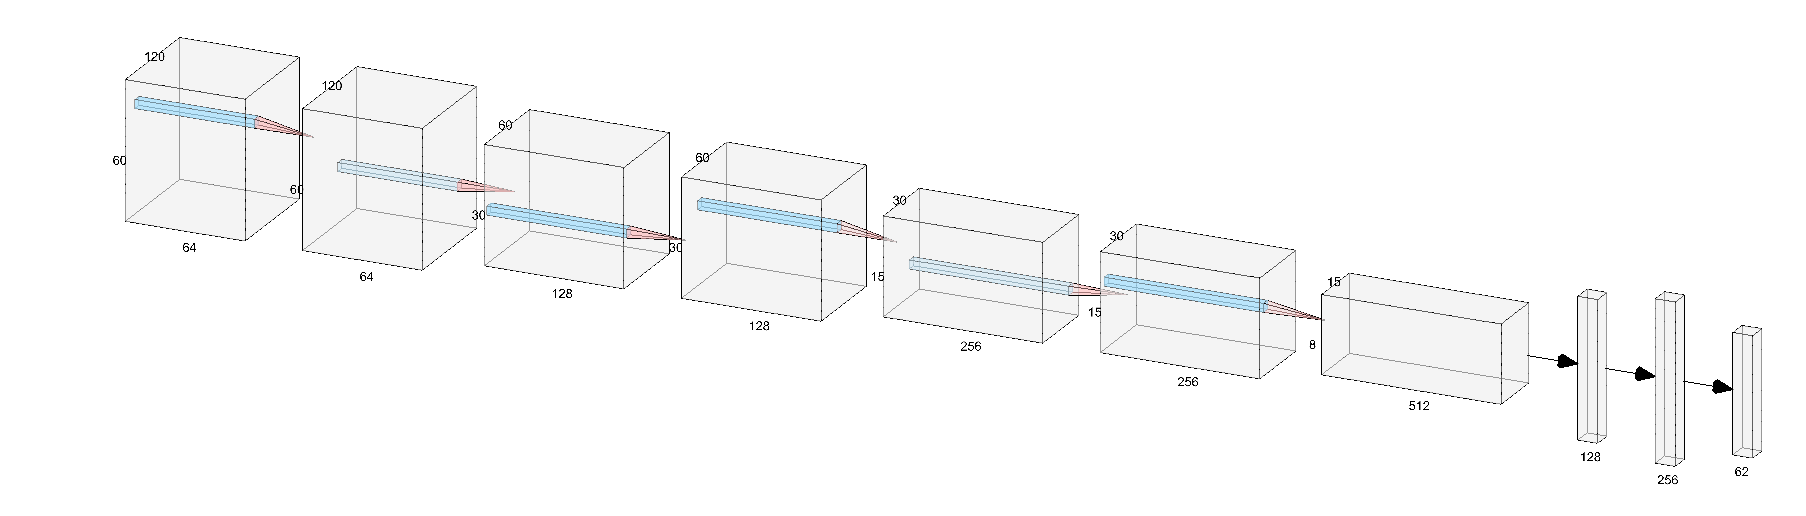
\includegraphics[width=\textwidth]{networks/big-2D-CNN-LSTM-Dense.png}
		\caption{Big 2D CNN with LSTM layer of size 128 and Dense layer of 256 neurons visualized with the chanel numbers omitted, to better visualize the volumetric layers, generated using \cite{nn-svg}}
		\label{figure:big-2D-CNN-LSTM-Dense}
	\end{figure}

	This network obtained better results than the initial CNN, with just an output dense layer, obtaining 73.7\% accuracy on the test and validation sets, but adding another dense layer to the CNN obtains better results, with 18\% higher accuracy. LSTM shows potential in classifying human gait.

	Taking from the previous result, maybe the CNN is to big and does not select all the relevant information for identifying people, so we changed the CNN with one that proved to have good results, from the 3D Convolution and adapted it to work with 2D input, removing the time dimension. The resulting CNN+RNN is described in Table~\ref{table:small-CNN-LSTM} and visually represented in Figure~\ref{figure:small-2D-CNN-LSTM-Dense}, with the chanel numbers included, because the convolutional layers are 2D, which are the most widespread and easy to represent visually.

	\begin{table}[h]
		\centering
		\renewcommand{\arraystretch}{1.5}

		\caption{Description of the CNN+RNN Model with fewer Convolution layers}
		\label{table:small-CNN-LSTM}

		\begin{tabularx}{\textwidth}{XXXX}
			\textbf{Layer name} & \textbf{Size} & \textbf{No. Filters} & \textbf{Activation} \\ \hline
			2D Convolution & 10, 10 & 32                   & elu                  \\ \hline
			2D Max Pooling & 2, 2   & \textbf{\textendash} & \textbf{\textendash} \\ \hline
			2D Convolution & 10, 10 & 16                   & elu                  \\ \hline
			2D Max Pooling & 2, 2   & \textbf{\textendash} & \textbf{\textendash} \\ \hline
			2D Convolution & 10, 10 & 8                    & elu                  \\ \hline
			2D Max Pooling & 2, 2   & \textbf{\textendash} & \textbf{\textendash} \\ \hline
			2D Convolution & 10, 5  & 4                    & elu                  \\ \hline
			2D Max Pooling & 2, 2   & \textbf{\textendash} & \textbf{\textendash} \\ \hline
			LSTM           & 128    & \textbf{\textendash} & tanh, sigmoid        \\ \hline
			Dense          & 256    & \textbf{\textendash} & elu                  \\ \hline
			Dense          & 62     & \textbf{\textendash} & softmax              \\
		\end{tabularx}
	\end{table}

	\begin{figure}
		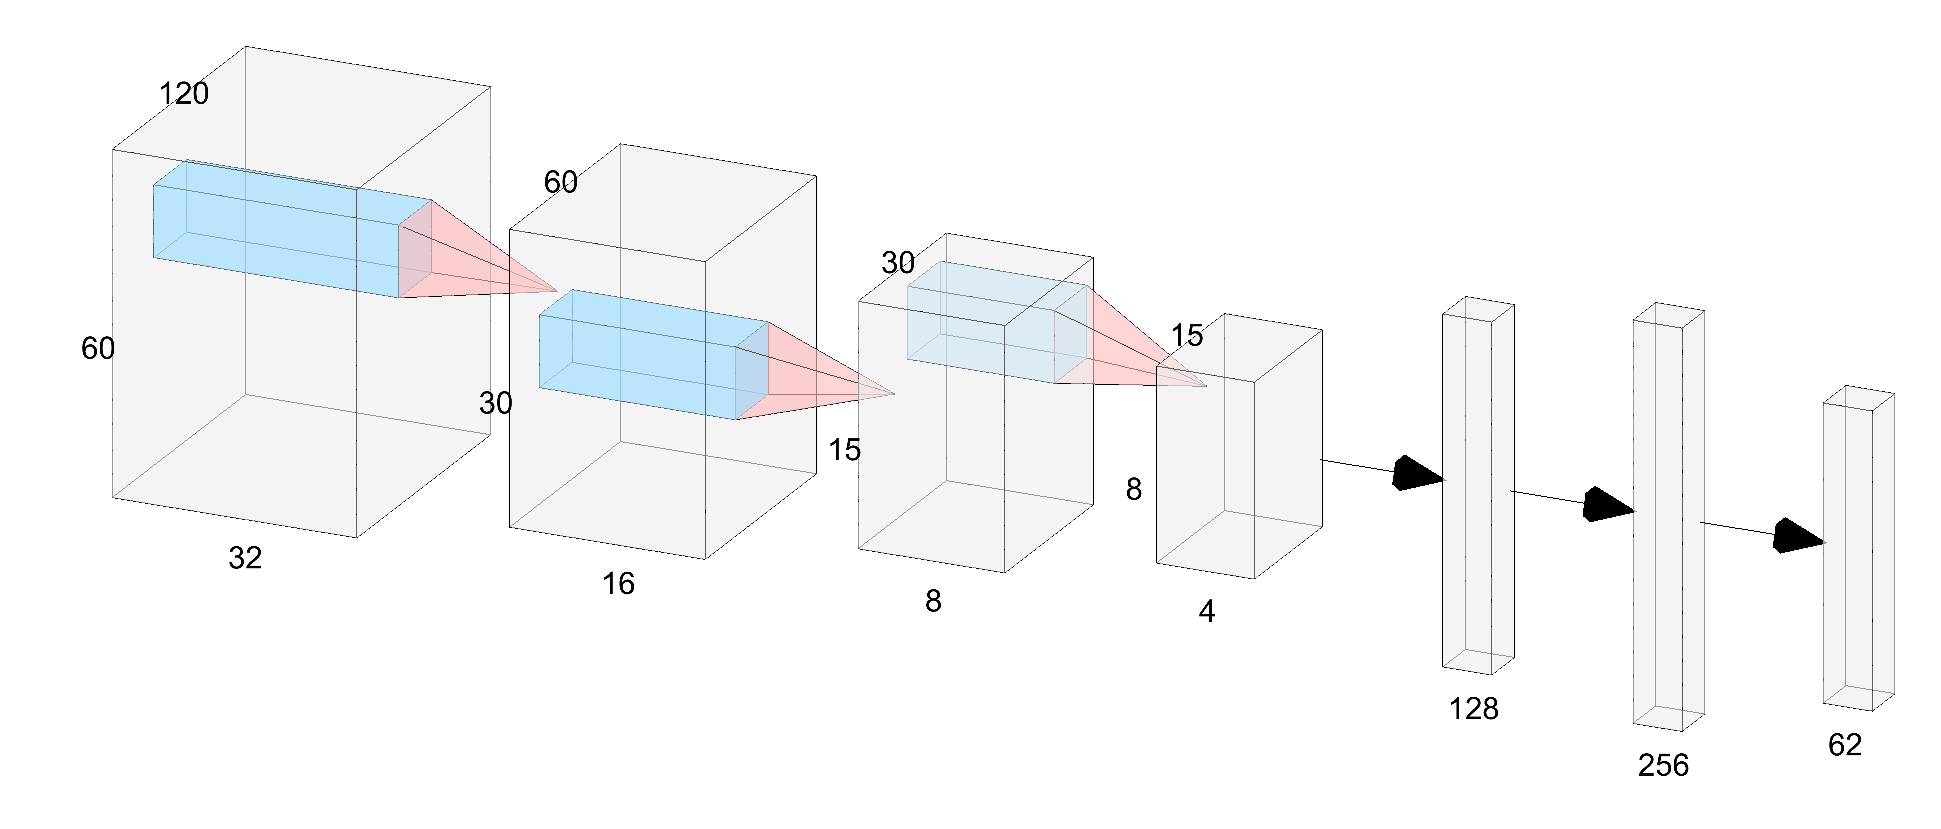
\includegraphics[width=\textwidth]{networks/small-2D-CNN-LSTM-Dense.png}
		\caption{Small 2D CNN with LSTM layer of size 128 and Dense layer of 256 neurons visualized with the chanel numbers omitted, to better visualize the volumetric layers, generated using \cite{nn-svg}}
		\label{figure:small-2D-CNN-LSTM-Dense}
	\end{figure}

	Using a smaller CNN did not improve the accuracy by much, to 74\%, on validation and testing, so the Convolution network does not matter how big it is. Further tests in which we increase the size of the LSTM layer will be done, to se how it affects the classification performance.

	To prevent overfitting we have used early stopping and adding dropout to all the layers, except the input layer. If the network did not obtain a better accuracy on the validation set than the best recorded yet, in 20 epochs, we stopped the training and run the best model on the testing set. Dropout picks at random a number of nodes, in the current layer, which will be used, so that all the nodes have equal chances to have their output evaluated and not overridden by other nodes on the same layer. In our models we chose to use a dropout on half of our nodes on each layer. Learning was speedup using the Adam optimization.

	After obtaining these result we tied specializing the model for the $90^\circ$ viewing angle, using the already trained model on all the angles and further training it on only one angle. This obtained an improvement in classification accuracy, reaching 79\%. It did not manage to outperform the 3D Convolution model, but it shows potential for specialization on only one viewing angle.

	\clearpage

	\section{Conclusions}
	\vspace{1cm}

	Human gait recognition using machine vision aims to identify humans based on their walking style and manner in a non intrusive manner. This paper covers a couple of approaches using Deep Neural Networks to identify people by their gait, using 3D Convolutional Neural Networks or Convolutional Recurrent Neural Networks, with varying degrees of success. One model proved to obtain competitive performance.

	All the models have been trained, validated and tested using all the 11 available angles, for each person, from the first half of the CASIA-B data set. Comparing all the approaches described we obtain the following results, shown in Table~\ref{table:all-results}, with the models sizes shown in Table~\ref{table:all-size}, and find that the Model-Free approaches have learned useful features for classification and of those ones the 3D Convolutional Neural Network performed the best, obtaining an accuracy of 91.7\% on testing. Keep in mind that all the inputs have been normalized and sanitized for the neural networks.

	\begin{table}[h]
		\centering
		\renewcommand{\arraystretch}{1.5}

		\caption{Comparison of the size of all the approaches}
		\label{table:all-size}

		\begin{tabular}{ll}
			\textbf{Model name}  &\textbf{Parameters} \\ \hline
			Shape Index + 3D CNN & $\approx 650.000$   \\ \hline
			3D CNN               & $\approx 650.000$   \\ \hline
			2D Deep CNN + LSTM   & $\approx 5.100.000$ \\ \hline
			2D CNN + LSTM        & $\approx 250.000$   \\ \hline
			3D CNN + Dense(200)  & $\approx 650.000$   \\
		\end{tabular}
	\end{table}

	\begin{table}[h]
		\centering
		\renewcommand{\arraystretch}{1.5}

		\caption{Comparison of all the approaches on the test data set}
		\label{table:all-results}

		\begin{tabularx}{\textwidth}{X|X|X|X|X|X}
			\textbf{View Angle} & \textbf{Shape Index + 3D CNN} & \textbf{3D CNN} & \textbf{2D Deep CNN + LSTM} & \textbf{2D CNN + LSTM} & \textbf{3D CNN + Dense(200)}\\ \hline
			All angles  & 1.62\%               & 59\%                 & 73.7\% & 74\%   & 91.7\% \\ \hline
			$0^\circ$   & \textbf{\textendash} & \textbf{\textendash} & 55.7\% & 57.3\% & 88.5\% \\ \hline
			$18^\circ$  & \textbf{\textendash} & \textbf{\textendash} & 62.9\% & 67.7\% & 93.5\% \\ \hline
			$36^\circ$  & \textbf{\textendash} & \textbf{\textendash} & 70.9\% & 64.5\% & 90.3\% \\ \hline
			$54^\circ$  & \textbf{\textendash} & \textbf{\textendash} & 74.1\% & 77.4\% & 93.5\% \\ \hline
			$72^\circ$  & \textbf{\textendash} & \textbf{\textendash} & 83.8\% & 80.6\% & 93.5\% \\ \hline
			$90^\circ$  & \textbf{\textendash} & 89\%                 & 80.6\% & 83.8\% & 91.9\% \\ \hline
			$108^\circ$ & \textbf{\textendash} & \textbf{\textendash} & 85.4\% & 82.2\% & 91.9\% \\ \hline
			$126^\circ$ & \textbf{\textendash} & \textbf{\textendash} & 77.4\% & 77.4\% & 93.5\% \\ \hline
			$144^\circ$ & \textbf{\textendash} & \textbf{\textendash} & 80.6\% & 66.1\% & 93.5\% \\ \hline
			$162^\circ$ & \textbf{\textendash} & \textbf{\textendash} & 70.9\% & 70.9\% & 88.7\% \\ \hline
			$180^\circ$ & \textbf{\textendash} & \textbf{\textendash} & 67.7\% & 64.5\% & 90.3\% \\
		\end{tabularx}
	\end{table}

	From the results presented above we can say that using and representing time as an additional dimension in the input for Convolutional Neural Networks, calculating convolution over tree dimensions, obtain better accuracy than usual two dimensional convolution using internal memory from a Recurrent Neural Network. It may be because the differences between different frames, from the same input sequence, are to small and the LSTM nodes confuse or chose to not remember some relevant past features, whereas in convolution features are combined together of filtered out if there are not as good descriptors as others. When testing only for one view angle, $90^\circ$, the results are not much better for the 3D CNN + Dense model, but our other model had improved considerably, especially the simple 3D CNN, from 59\% to 89\%, a 30 points increase, showing us that indeed this model lacked power in classification, when dealing with multiple view angles.

	When testing on individual angles we see that the accuracy does not vary wildly from angle to angle, for the 3D CNN with Dense, which shows that it generalizes well, but the LSTM models have better precision on the angles closest to $90^\circ$ and the ones closes to $0^\circ$ or $180^\circ$ do considerably worse, a decrease from 83.8\% to 57.3\%, 64.5\% respectively. From the result in Table~\ref{table:all-results} we can conclude that the Recurrent Neural Networks we designed have poor generalization power, compared to the 3D Convolution Neural Networks.

	When comparing with existing approach we also see that when the classification algorithm is left alone to extract the best features to utilize outperform the ones in which the features are already extracted using image processing algorithms. In Munif Alotaibi and Ausif Mahmood \cite{gait-with-gei} they obtain 98.3\% on the normal clothes data set, using only the 90 degrees viewing angle, where the best we obtained 91.9\%, whereas Hazem El-Alfy, Ikuhisa Mitsugami and Yasushi Yagi \cite{gait-with-curvature-map} obtain 16.7\%, for the same viewing angle. Munif Alotaibi and Ausif Mahmood represented the information gained from the passing of time by combining all the silhouette frames into one, using Gait Energy Image (GEI) \cite{gei}, on the other hand Hazem El-Alfy, Ikuhisa Mitsugami and Yasushi Yagi extracted curvature information from frames composing a full gait cycle and passed it to a classification algorithm. A comparison with other approaches can be found in Table~\ref{table:camparison-results}.

	\begin{table}[h]
		\centering
		\renewcommand{\arraystretch}{1.5}

		\caption{Comparison of our best two approaches with other existing results}
		\label{table:camparison-results}

		\begin{tabularx}{\textwidth}{X|X|X|X|X|X|X}
			\textbf{View Angle} & \textbf{VGR-net \cite{VGR-Net}} & \textbf{MVCNN \cite{Wolf2016MultiviewGR}} & \textbf{MDM \cite{gait-with-curvature-map}} & \textbf{GEI deep CNN \cite{gait-with-gei}} & \textbf{2D CNN + LSTM} & \textbf{3D CNN + Dense(200)}\\ \hline
			All angles  & \textbf{\textendash} & \textbf{\textendash} & \textbf{\textendash} & \textbf{\textendash} & 74\%   & 91.7\% \\ \hline
			$0^\circ$   & 98.33\%              & 96.3\%               & 99.5\%               & \textbf{\textendash} & 57.3\% & 88.5\% \\ \hline
			$18^\circ$  & 99.17\%              & 98.2\%               & 80.7\%               & \textbf{\textendash} & 67.7\% & 93.5\% \\ \hline
			$36^\circ$  & 99.17\%              & 98.5\%               & 31.5\%               & \textbf{\textendash} & 64.5\% & 90.3\% \\ \hline
			$54^\circ$  & 96.67\%              & 95.4\%               & 21.2\%               & 71.5\%               & 77.4\% & 93.5\% \\ \hline
			$72^\circ$  & 97.92\%              & 94.3\%               & 16.1\%               & \textbf{\textendash} & 80.6\% & 93.5\% \\ \hline
			$90^\circ$  & 97.08\%              & 99.9\%               & 16.7\%               & 69.0\%               & 83.8\% & 91.9\% \\ \hline
			$108^\circ$ & 97.91\%              & 98.6\%               & 12.6\%               & \textbf{\textendash} & 82.2\% & 91.9\% \\ \hline
			$126^\circ$ & 97.08\%              & 97.0\%               & 14.9\%               & 80.0\%               & 77.4\% & 93.5\% \\ \hline
			$144^\circ$ & 96.25\%              & 97.4\%               & 24.3\%               & \textbf{\textendash} & 66.1\% & 93.5\% \\ \hline
			$162^\circ$ & 96.67\%              & 99.2\%               & 33.0\%               & \textbf{\textendash} & 70.9\% & 88.7\% \\ \hline
			$180^\circ$ & 97.08\%              & 96.1\%               & 55.1\%               & \textbf{\textendash} & 64.5\% & 90.3\% \\
		\end{tabularx}
	\end{table}

	From Table~\ref{table:camparison-results} we can see that when training on all the angles, and not for a specific one, it tends to have worse result, but in exchange we obtain the possibility to use only one model to identify persons from any angle, and do not need them to walk in a specific direction or use another model/algorithm to identify the angle and use the model used on that specific angle, or a small range of closely related angles.

	Also that we can see that a relatively simple network, with 3D Convolution layers followed by Pooling which halves the size in all dimensions, that steadily decrease in size and a small dense layer at the end perform comparably with the best result in the field.

	Based on the results presented above there is no need to do heavy preprocessing of the input to help the neural network obtain a better classification performance, it even impedes the performance of the classification algorithm, compared to neural network with just the silhouettes or the silhouettes with additional information. Deep Convolutional Neural Networks are very powerful in learning using temporal data as an additional dimension of the input, even thou it does not span only for short periods of time.

	\clearpage

	\section{Bibliography}
	\bibliography{bibliografie}
	\bibliographystyle{ieeetr}

\end{document}
